

\documentclass[color=usenames,dvipsnames]{beamer}

\usepackage[adobefonts,noindent]{ctex} %中文支持
\setCJKmainfont{SimSun}

\mode<presentation> {

\usetheme{Madrid}
\usecolortheme{lily}
\useoutertheme{infolines}

}


\usepackage{booktabs}
\usepackage{tikz}

% for color
\newcommand{\setof}[1]{\ensuremath{\left \{ #1 \right \}}}
\newcommand{\tuple}[1]{\ensuremath{\left \langle #1 \right \rangle }}
\newcommand{\red}[1]{\textcolor{red}{#1}}
\newcommand{\brown}[1]{\textcolor{brown}{#1}}
\newcommand{\green}[1]{\textcolor{green}{#1}}
\newcommand{\blue}[1]{\textcolor{blue}{#1}}
\newcommand{\cyan}[1]{\textcolor{cyan}{#1}}

% for gif
% \usepackage[dvipdfmx]{movie15}
\usepackage{graphicx}
\usepackage{animate}
\usepackage{media9}

% Thin fonts
\usepackage{cmbright}
\usepackage[T1]{fontenc}

\definecolor{dark_grey}{gray}{0.5}
\setbeamercolor{normal text}{fg=dark_grey,bg=white}
\setbeamertemplate{navigation symbols}{}

\setbeamercolor*{palette primary}{fg=gray!100,bg=gray!10}
\setbeamercolor*{palette quaternary}{fg=gray!100,bg=gray!10}
\setbeamercolor*{palette secondary}{fg=gray!100,bg=gray!20}
\setbeamercolor*{palette tertiary}{fg=gray!100,bg=gray!10}
\setbeamercolor*{navigation symbols}{fg=white,bg=white}
\usefonttheme{default}


\setbeamertemplate{blocks}[rounded][shadow=false]
\setbeamercolor{block title}{bg=gray!10}
\setbeamercolor{block body}{fg=gray,bg=gray!10}
%\setbeamercolor{frametitle}{fg=}

\setbeamertemplate{frametitle}[default][center]

\setbeamertemplate{itemize items}[default]
\setbeamertemplate{enumerate items}[default]

\newcommand{\F}{\mathbb{F}}


\title[2015 Summ]{2015秋季学期总结}
\author{韩喆}
\institute{PIE@WIP}
\date{2016-01-21}
\begin{document}


\begin{frame}
  \titlepage
\end{frame}

% Uncomment these lines for an automatically generated outline.
%\begin{frame}{Outline}
%  \tableofcontents
%\end{frame}

\begin{frame}


\section{Introduction}
\frametitle{工作简介}
\begin{itemize}
\item  助教:冯老师开的2015级工学院《计算概论》
\item \color{Green}
 组会报告:大组会2次+小组会2次
\item\color{RedOrange} 实验室新主页
\color{blue}
\item 结构化知识库构建+展示
\end{itemize}
\end{frame}


\begin{frame}{助教}
 \begin{block}{}
  2015级工学院计算概论
 \end{block}

 \begin{itemize}
  \item 和吕超、李友焕师兄担任助教
  \item 每周一下午的上机辅导
  \item 两次课堂答疑/习题课,期中/期末监考,阅卷
 \end{itemize}

 \pause
 感想
 \begin{itemize}
  \item 感觉回到了本科的时候(但是没有绩点的压力了)
  \item 编程能力还有待提高
 \end{itemize}
\end{frame}

\begin{frame}{组会报告}
 \begin{block}{大组会}
  \begin{itemize}
   \item EMNLP 2015 的一篇做不同知识库的合并工作的文章
   \only<1>{
    \begin{itemize}
     \item Knowledge Base Unification via Sense Embeddings and Disambiguation
     \item 合并实体、合并谓词
    \end{itemize}
    }
   \item 目前工作:中文知识库构建
   \only<1>{
    \begin{itemize}
     \item 构建自己的\begin{color}{blue}类别\end{color}和\begin{color}{red}谓词\end{color}集合
    \end{itemize}
    }
  \end{itemize}
 \end{block}


 \only<2-3>{
 \begin{block}{小组会}
  \begin{itemize}
   \item 介绍了几个自己在用的工具/软件和一篇利用关联规则查找spo中的相同谓词
   \only<2>{
    \begin{itemize}
     \item Synonym Analysis for Predicate Expansion
    \end{itemize}
    }
   \item 利用RNN提取文本中的关系向量,和KB结合,训练更好的实体向量、关系向量
   \only<2>{
      \begin{itemize}
       \item EMNLP 2015: Representing Text for Joint Embedding of Text and Knowledge Bases
      \end{itemize}
      }
  \end{itemize}
 \end{block}
 }
\end{frame}

\begin{frame}{实验室新主页}
\begin{columns}
 \column{0.5\hsize}
 \begin{itemize}\small
  \item 首页:中英文 (感谢贺文强、罗炳峰)
  \only<2->{\item 新闻:markdown -> html}
  \only<3->{\item 团队:老师的详细信息+学生的基本信息}
 \end{itemize}
 \vspace{1cm}
 \only<2->{\centering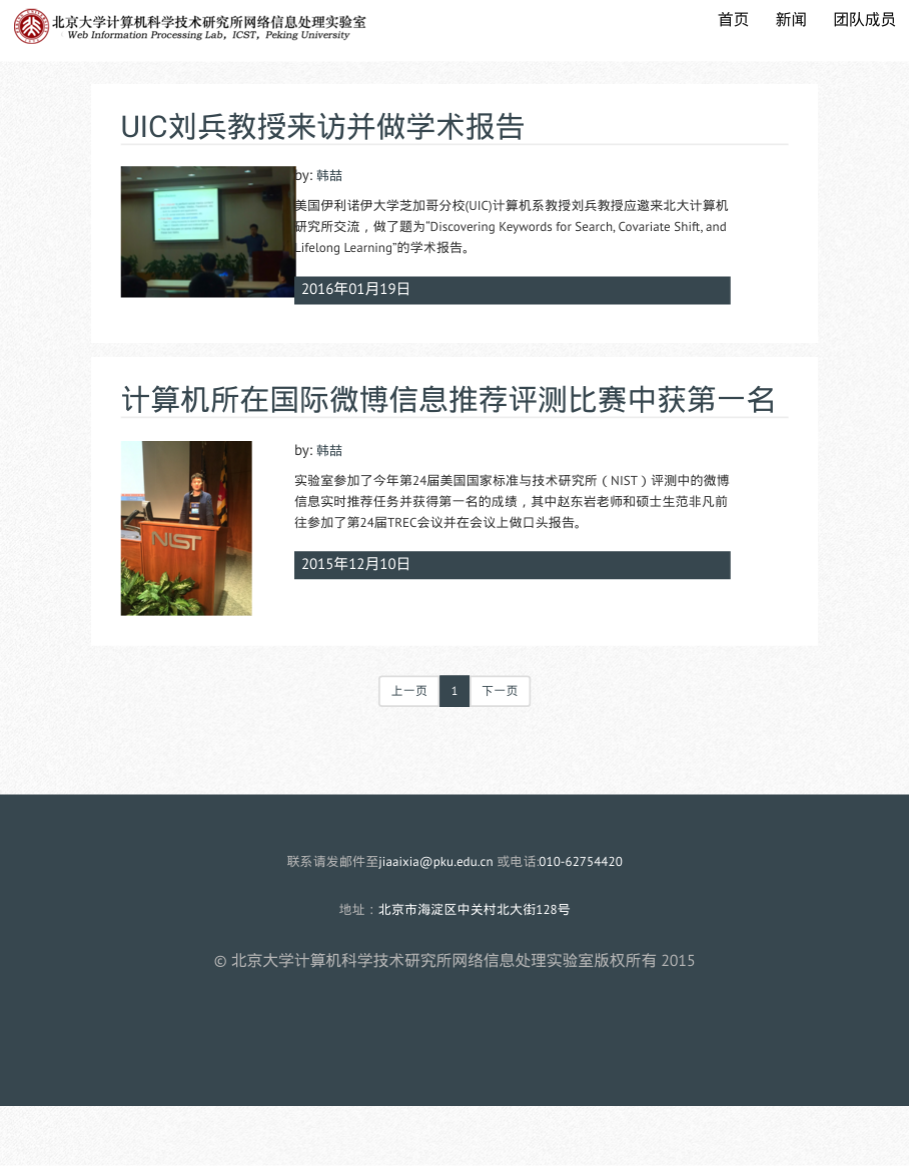
\includegraphics[width=0.5\hsize]{pic/wip-news.png}}

 \column{0.15\hsize}
 \centering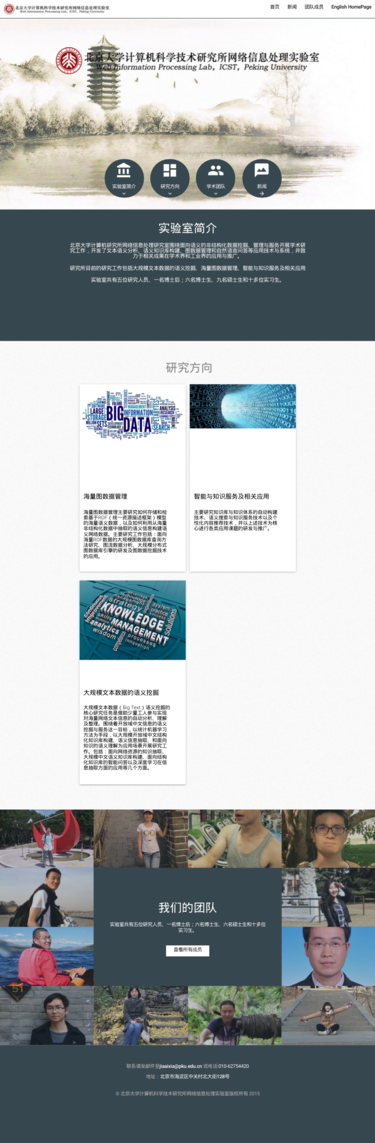
\includegraphics[height=0.7\textheight]{pic/wip-homepage15.png}
 \column{0.3\hsize}
 \only<3->{\centering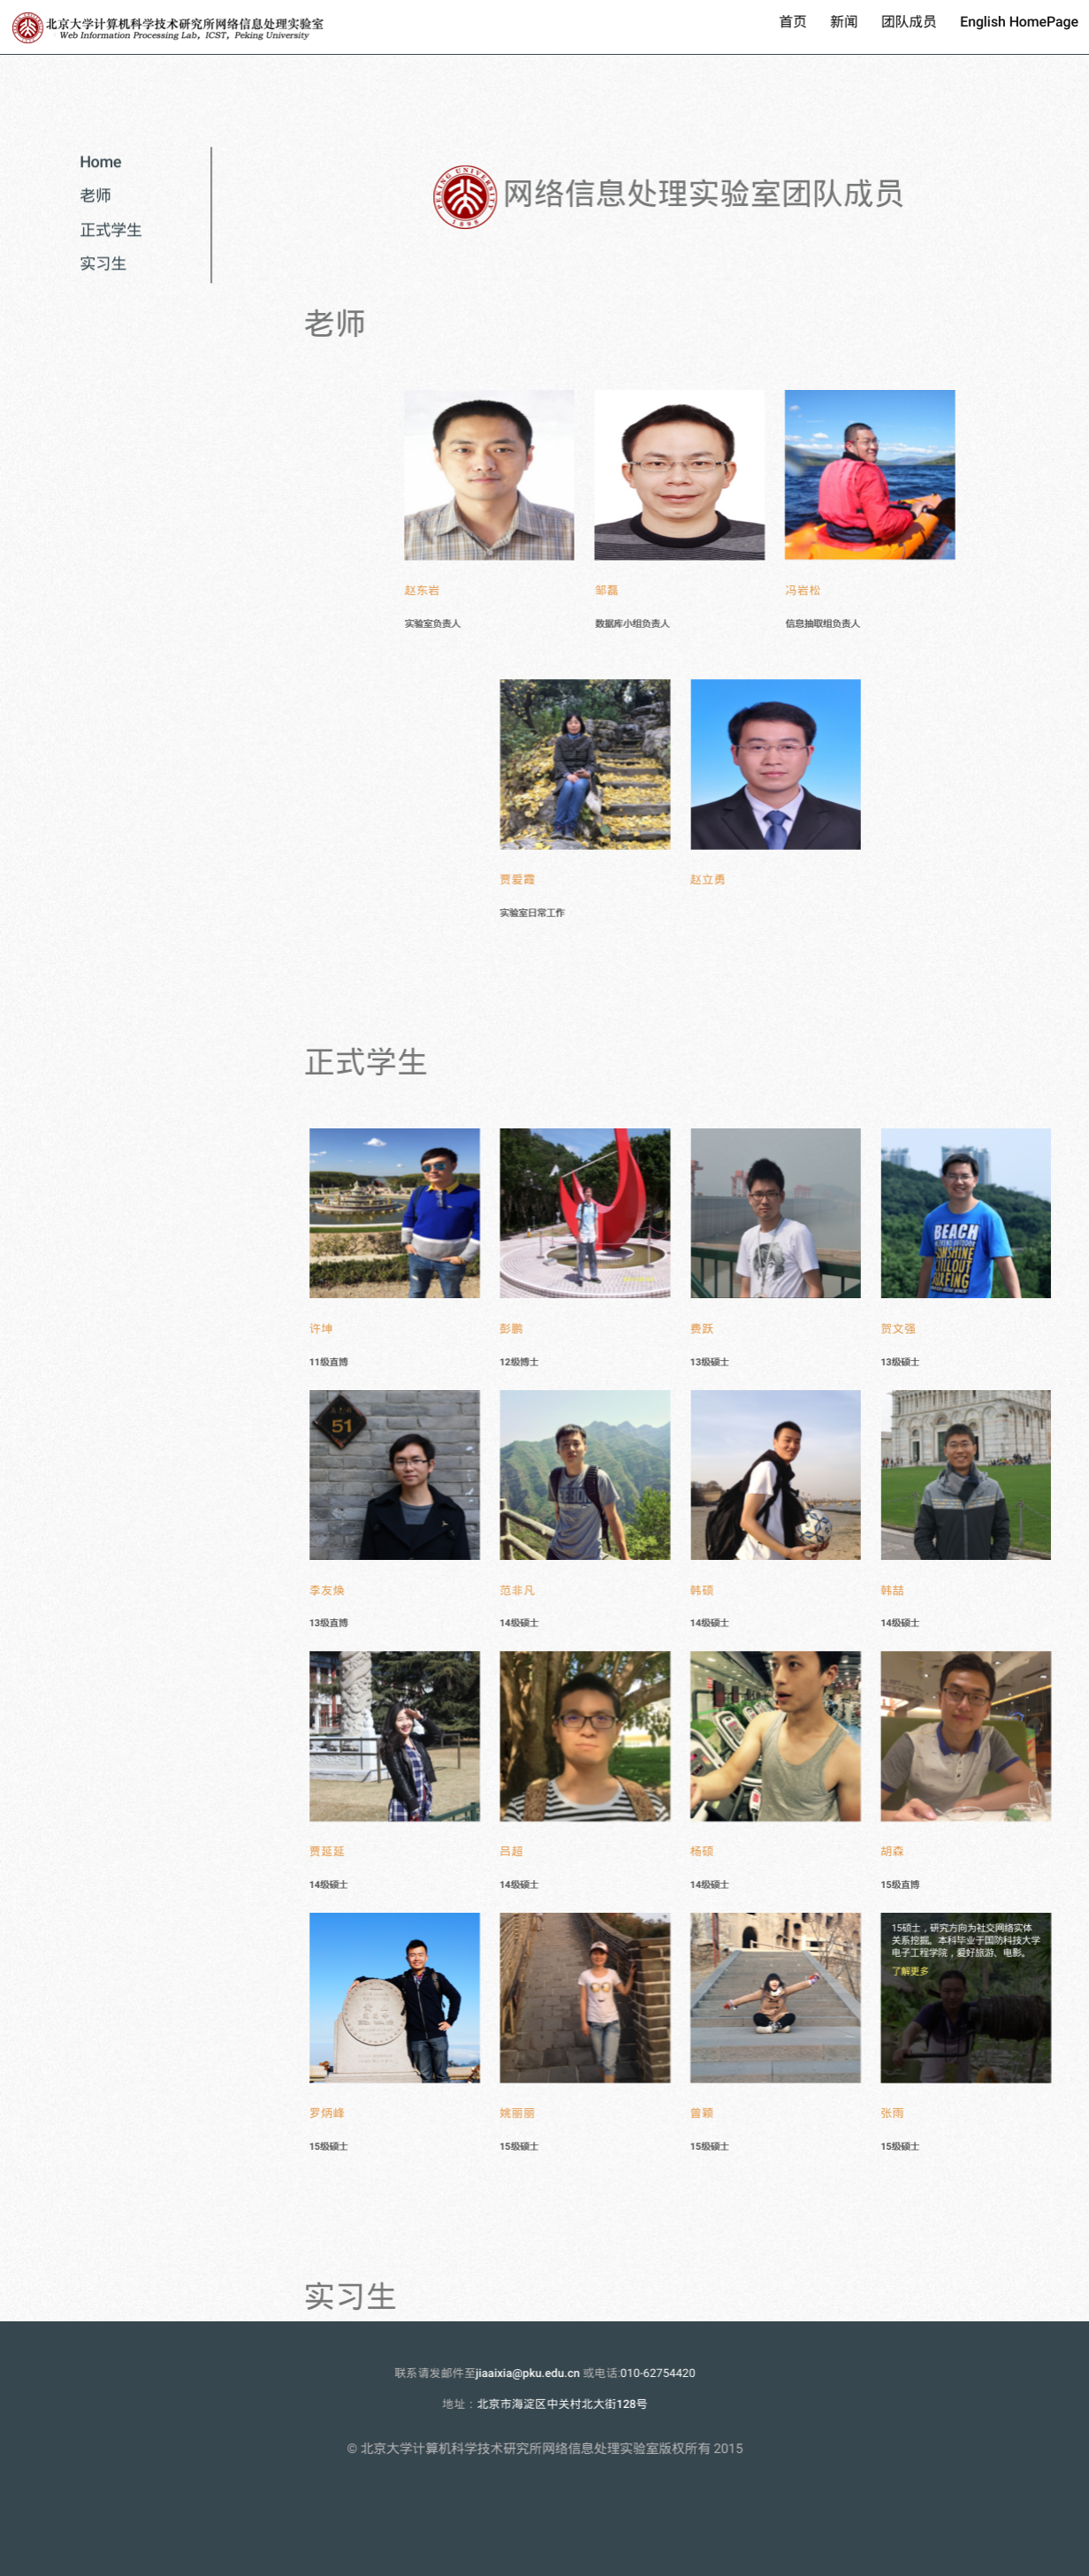
\includegraphics[height=0.7\textheight]{pic/wip-team.png}}
\end{columns}
\end{frame}

\begin{frame}{结构化知识库构建}
 \begin{itemize}\small
  \item 之前大组会做过短报告,目前已经形成了基本的类别体系(和\red{贺易之、郑军祥}合作),谓词体系待完成
    \begin{itemize}
     \item 谓词对齐的工作和冯老师讨论了一个新的方法来做,用以修改之前的论文
    \end{itemize}
  \item 最近(和\red{蔡少峰}师弟合作)做了一些demo展示抽取的三元组、实体类别
 \end{itemize}
\end{frame}

\begin{frame}{demo}
\begin{columns}
 \column{0.5\hsize}
\centering\animategraphics[loop,height=0.45\textheight]{4}{pic/ontology/ontology-}{0}{56}
 \column{0.5\hsize}
\centering\animategraphics[loop,height=0.45\textheight]{4}{pic/triple/tri-}{0}{406}
\end{columns}
 \begin{itemize}\footnotesize
  \item 左:显示每个类别/子类别覆盖实体数量
  \item 右:查询实体的关系图
 \end{itemize}

\end{frame}

\begin{frame}{总结}
 \begin{itemize}
  \item 做的事情比较杂,导致科研效率较低,压力比较大
    \begin{itemize}
     \item 实验室网站的事情暂时告一段落,会专注时间做知识库的构建工作
    \end{itemize}
  \item 在不断尝试一些新的技术、工具,多做一些有意思的东西
  \item 要开始为找工作做准备了,刷题,看书...
 \end{itemize}
\end{frame}


\frame{
  \begin{columns}[c]
   \column{.2\hsize}
   \column{.6\hsize}
   \begin{block}{}
    \centering \Large 谢谢大家!
   \end{block}

   \column{.2\hsize}
  \end{columns}

}
\end{document}
